\subsection{Amorfización del silicio mediante un templado simulado y análisis de la función de distribución radial (RDF)}\label{s:rdfb}

\begin{figure}[h!]
    \centering
    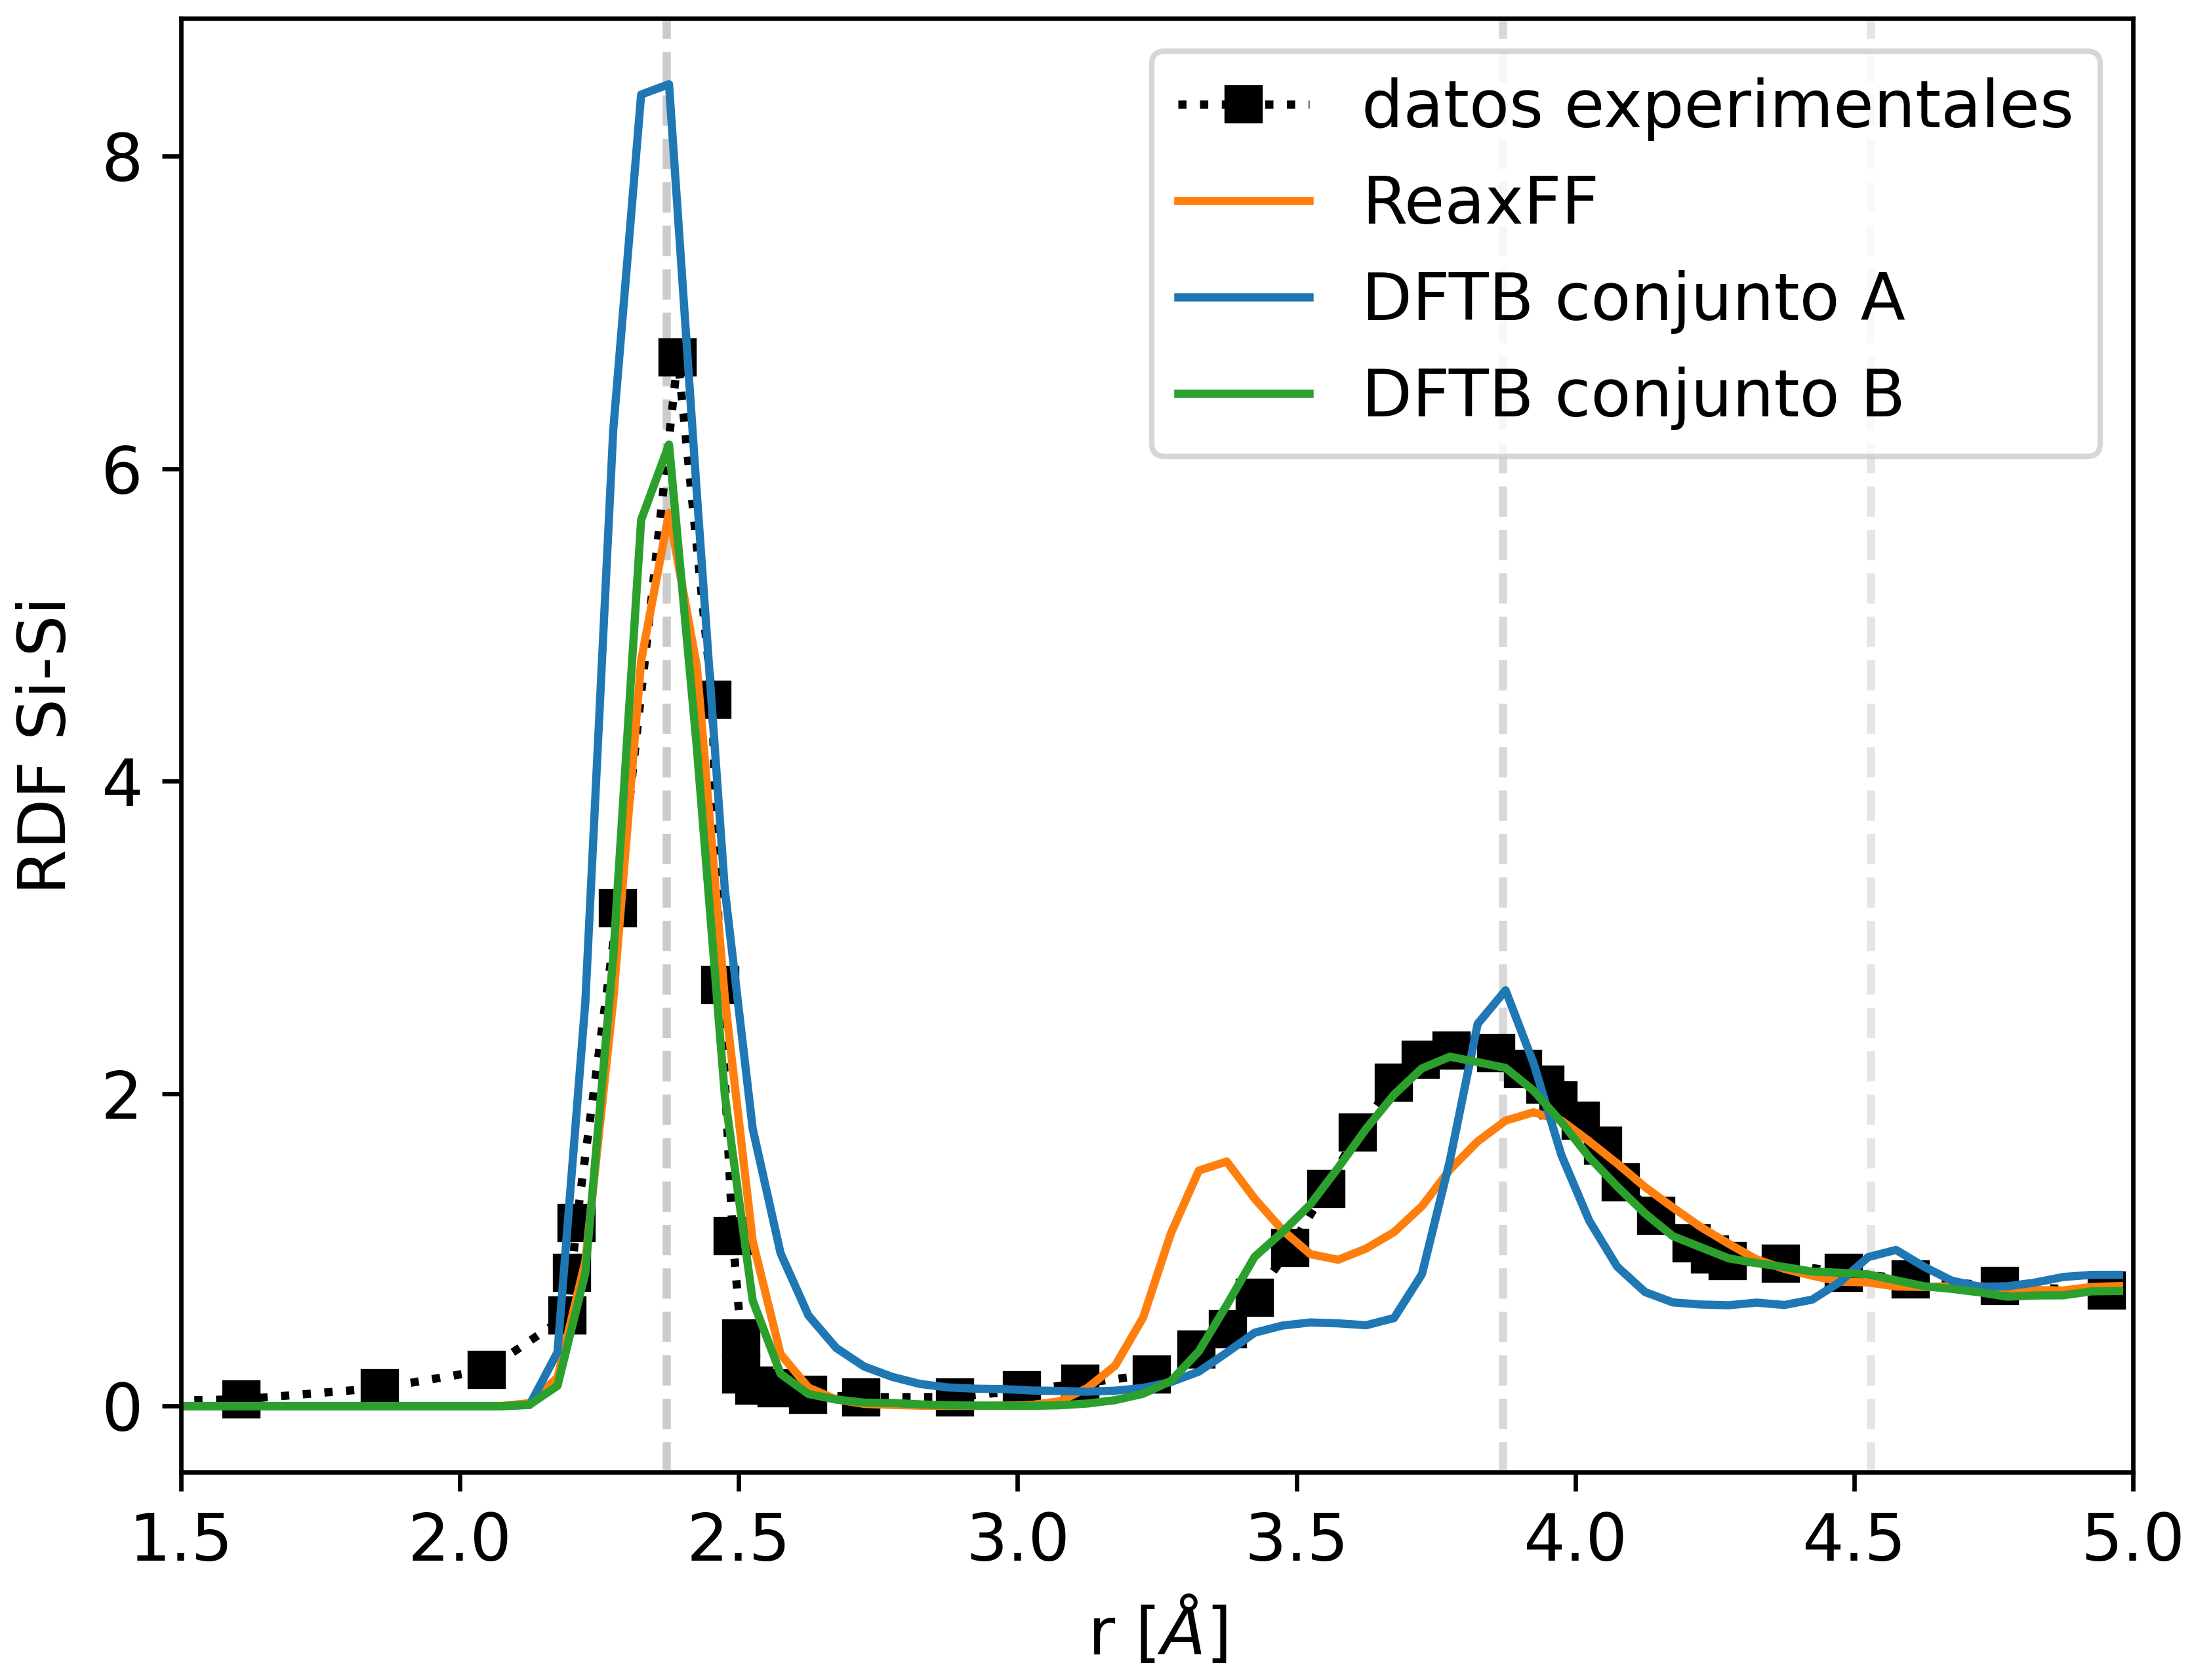
\includegraphics[width=.7\textwidth]{Silicio/modelo/resultados/rdf/rdf.png}
    \caption{Función de distribución radial (RDF) de silicio amorfo para los
    conjuntos A y B de parametrizaciones. Los resultados se comparan con 
    mediciones de la referencia \cite{laaziri1999} y con los resultados obtenidos
    utilizando el ReaxFF \cite{fan2013}. Las líneas grises discontinuas verticales
    muestran dónde estarían los picos del silicio cristalino a 0 K. Se encuentra 
    una concordancia excelente entre el experimento y la parametrización del 
    conjunto B.}
    \label{fig:rdfb}
\end{figure}

Por último, las mayores discrepancias entre las energías de formación calculadas con DFTB
con respecto a DFT se corresponden a estructuras de silicio amorfo, por lo cual,
se realizó una evaluación extra para este caso. En la Figura \ref{fig:rdfb} se 
muestran las RDFs Si-Si obtenidas por un templado simulado para cada una de las
parametrizaciones. Además, se compara con el potencial previo de ReaxFF 
\cite{fan2013} y con una determinación experimental \cite{laaziri1999}. Para 
obtener las estructuras amorfas se comenzó con una celda de c-Si con 64 átomos 
a la cual se le realizó un templado simulado en el ensamble $NVT$ utilizando el 
termostato de Nosé-Hoover. El mismo consistió en una etapa inicial de 
calentamiento lineal desde temperatura ambiente hasta 3000 K durante 100 ps, luego una
termalización a dicha temperatura por 600 ps y, por último, un enfriamiento 
exponencial de 600 ps hasta llegar a temperatura ambiente. Para todas las etapas
se utilizó un paso temporal de 1 fs. Para el cómputo de las RDFs que se muestran
en la Figura \ref{fig:rdfb} se equilibró la estructura alcanzada a temperatura 
ambiente durante 100 ps. Puede destacarse que los resultados del conjunto B de parámetros muestran
una concordancia excelente con los datos experimentales de la referencia 
\cite{laaziri1999}, lo que convierte a esta parametrización en la más adecuada
para simulaciones futuras. Los archivos de dichos parámetros están disponibles
en un repositorio público \cite{dftb_lisi}.
